\documentclass[9pt, xcolor=table]{beamer}

\usepackage[utf8]{inputenc}
\usepackage[round, comma]{natbib}
\usepackage{amsmath}
\usepackage{hyperref}
\usepackage{amsfonts}
\usepackage{verbatim}
\DeclareMathOperator*{\argmin}{arg\,min}



\mode<presentation> {

\usetheme{Madrid}

\setbeamertemplate{navigation symbols}{} 
\useinnertheme{circles}
\definecolor{greenish}{RGB}{0, 153, 76}
\usecolortheme[named=greenish]{structure}
}

\setbeamertemplate{headline}
{%
  \begin{beamercolorbox}[ht=3.5ex,dp=1.125ex,%
      leftskip=.3cm,rightskip=.3cm plus1fil]{section in head/foot}
    \usebeamerfont{section in head/foot}\usebeamercolor[fg]{section in head/foot}%
\insertsectionnavigationhorizontal{\paperwidth}{\hskip0pt plus1fill}{\hskip0pt plus1fill}
  \end{beamercolorbox}%
  \begin{beamercolorbox}[colsep=1.5pt]{middle separation line head}
  \end{beamercolorbox}
  \begin{beamercolorbox}[colsep=1.5pt]{lower separation line head}
  \end{beamercolorbox}
}

\title[Interpretation of black box models]{Interpretation of black box models using tree-based surrogate models \newline \small{Simulations}}
\author[Sofia Loibl]{Sofia Loibl}
\institute[LMU]{LMU München}
\date{\today}

\begin{document}

\begin{frame}
\titlepage 
\end{frame}


\section{Selection Bias}
\begin{frame}{Selection Bias}
\textbf{Goal:} 

Comparison of different versions of SLIM, MOB, CTree and GUIDE with respect to selection bias
\vspace{0.5cm}


\textbf{Selection bias:} 

An algorithm for recursive partitionig is called unbiased when, under the conditions of the null hypothesis of independence between a response $Y$ an covariates $X_{1},...X_{m}$ the probability of selecting covariate $X_{j}$ is $1/m$ for all $j = 1,...,m$ regardless of the measurement scales of number of missing values. \citep{Hothorn.2006}
\vspace{0.5cm}

\textbf{Measure:} p-value of a $\chi^2$ goodnes of fit test\\
H0: the probabilities of the population are all equal (or are equal to an assumed probability distribution p)
\vspace{0.5cm}

\textbf{Simulation Setting:} $1000$ simulation runs with $n= 1000$
\end{frame}




\begin{frame}{GUIDE}
Algorithm \citep{.2002}
\begin{enumerate}
    \item Fit regression model and determine signs of the residuals
    \item For each numerical variable divide data in 4 quartiles and construct a 2 × 4 contingency table with the signs of the residuals. For categorical variables the categories of the variable form the columns of the table. Calculate the p-value of the  $\chi^2$ independence test. (curvature test)
    \item For each pair of numerical variables divide the space of the two variables in four quadrants (use categories instead for categorical variables). Calculate the p-value of the  $\chi^2$ independence test. (interaction test)
    \item If the smallest p-value is from a curvature test, use the associated variable for splitting.
    \item If the smallest p-value is from an interaction test 
    \begin{enumerate}
        \item if both variables are numeric, perform splits at the mean value of both variables and use the variable, that yields to a smaller SSE
        \item if only one variable is categorical, use it as splitting variable
        \item if both are categorical, choose the one with the smaller curvature p-value.
    \end{enumerate}
\end{enumerate}
    
\end{frame}


\begin{frame}{Scenario Independence}
$X_{1}, X_{2} \sim U(0,1)$; 
$X_{3} \sim U(0,1)$ and rounded to one digit;
$X_{4}$ binary;
$X_{5}$ categorical with 5 levels;
$X_{6}$ categorical with 8 levels\\
$Y \sim N(0,1)$

\begin{figure}
    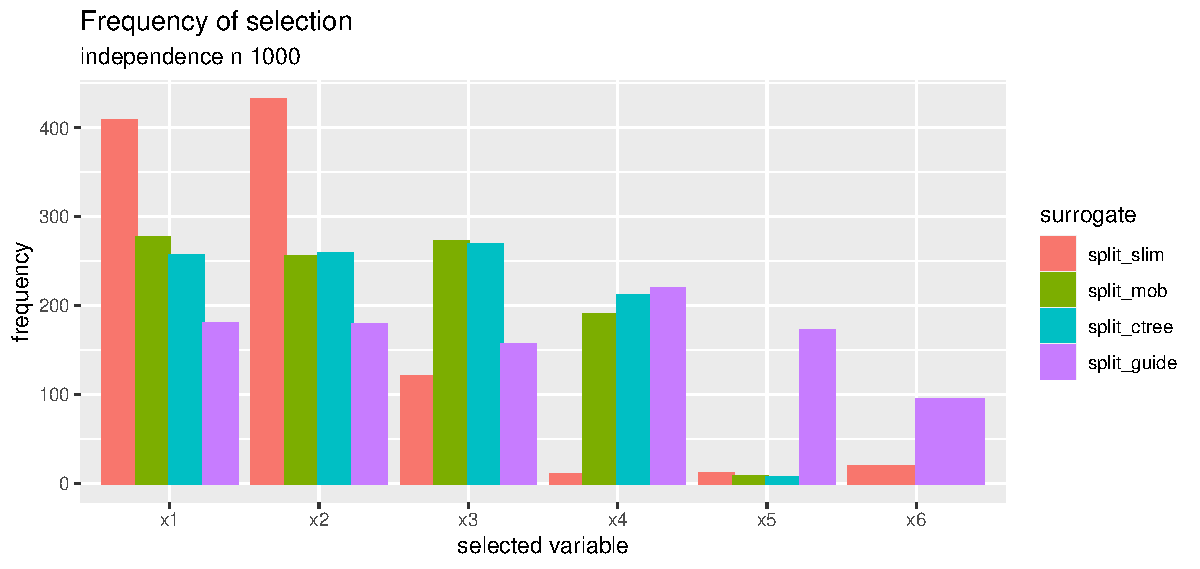
\includegraphics[width=11cm]{Figures/simulations/batchtools/selection_bias_general/independence_n1000.pdf}
\end{figure}
\end{frame}


\begin{frame}{Scenario Independence small}
All $X_j \sim U(0,1)$; $X_3$ rounded to one digit, $X_4$ rounded to two digits\\
$Y \sim N(0,1)$
\begin{figure}
    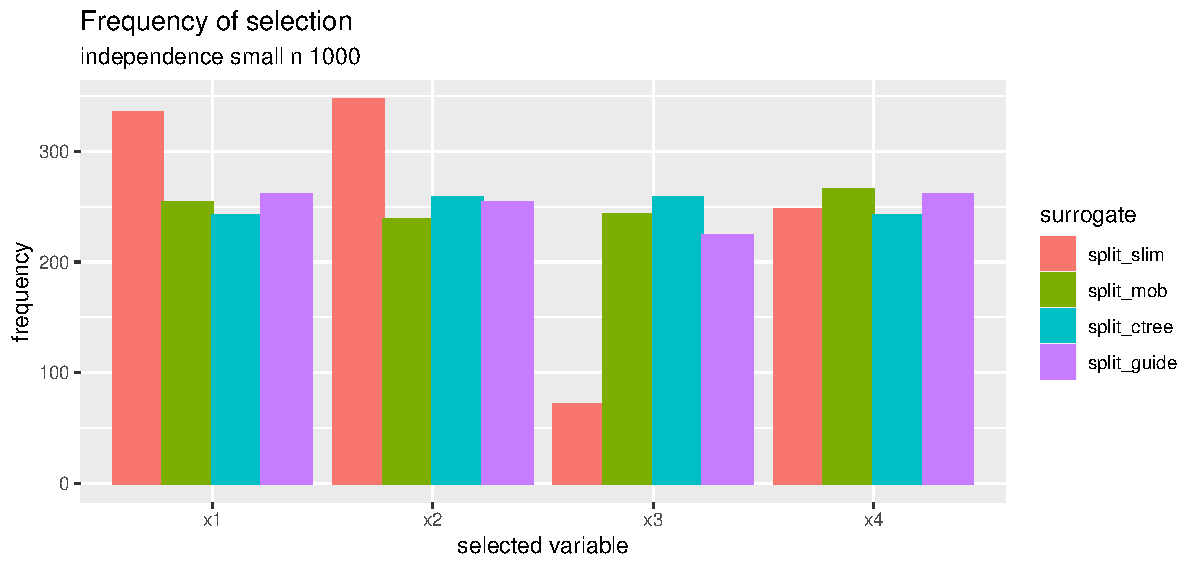
\includegraphics[width=10cm]{Figures/simulations/batchtools/selection_bias_general/independence_small_n1000.pdf}
\end{figure}

\begin{table}
\begin{tabular}[t]{r|r|r|r}
\hline
slim & mob & ctree & guide\\
\hline
$< 0.0001$ & $0.629 $ & $0.7954$ & $0.2914$\\
\hline
\end{tabular}
\caption{p-values of $X_^2$ goodness-of-fit test}
\end{table}

\end{frame}

\begin{frame}{Scenario Interaction}

All $X_j \sim U(0,1)$; $X_3$ rounded to one digit, $X_4$ rounded to two digits\\
$Y = X_1 + X_2 + X_3 + X_4 + X_1 X_2 + X_1 X_3 + X_1 X_4 + X_2 X_3 + X_2 X_4 + X_3 X_4 + eps$
\begin{figure}
    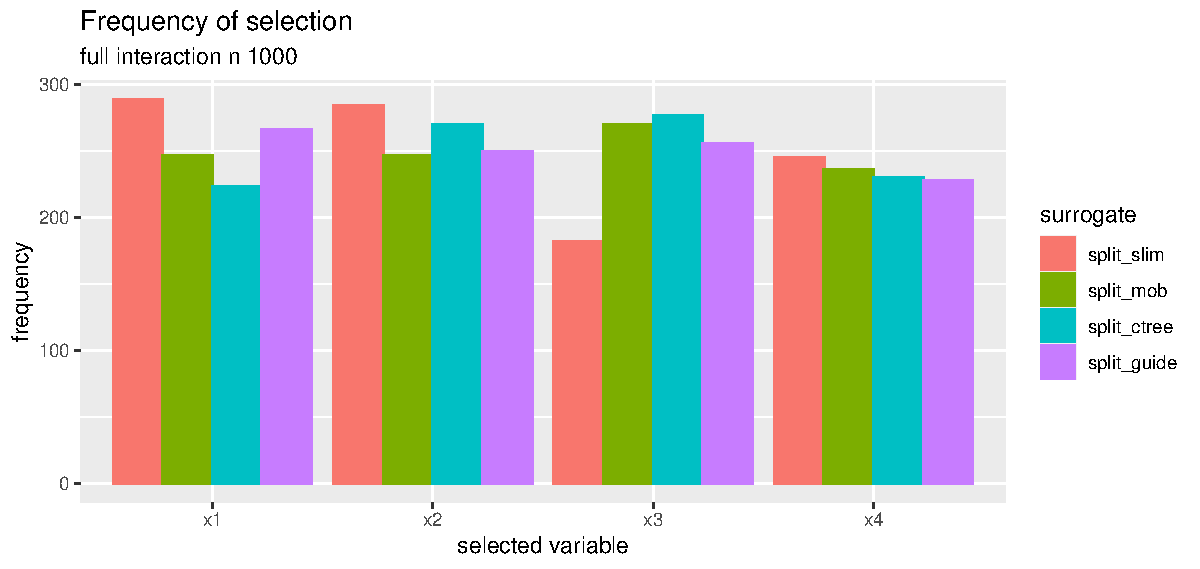
\includegraphics[width=10cm]{Figures/simulations/batchtools/selection_bias_general/full_interaction_n1000.pdf}
\end{figure}

\begin{table}
\centering
\begin{tabular}[t]{r|r|r|r}
\hline
slim & mob & ctree & guide\\
\hline
$ < 0.0001$ & $0.4833 $ & $0.0289$ & $0.3759$\\
\hline
\end{tabular}
\caption{p-values of $\chi_^2$ goodness-of-fit test}
\end{table}
\end{frame}

\begin{frame}{Influence of n.quantiles in SLIM on selection bias and performance}
All $X_j \sim U(0,1)$; $X_3$ rounded to one digit (10 possible quantiles), $X_4$ rounded to two digits (100 possible quantiles)\\
$Y = X_1 + X_2 + X_3 + X_4 + X_1 X_2 + X_1 X_3 + X_1 X_4 + X_2 X_3 + X_2 X_4 + X_3 X_4 + eps$

\begin{figure}
    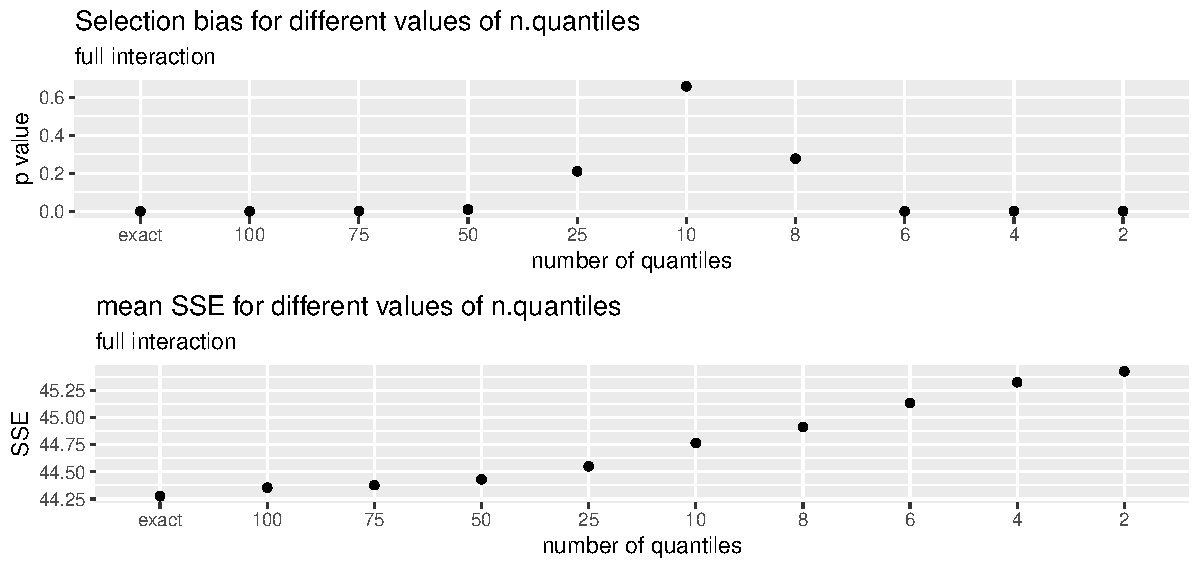
\includegraphics[width=10cm]{Figures/simulations/batchtools/selection_bias_slim/full_interaction.pdf}
\end{figure}

\end{frame}


\begin{frame}{Influence of n.quantiles in SLIM on selection bias and performance}
All $X_j \sim U(0,1)$; $X_3$ rounded to one digit, $X_4$ rounded to two digits\\
$Y \sim N(0,1)$
\begin{figure}
    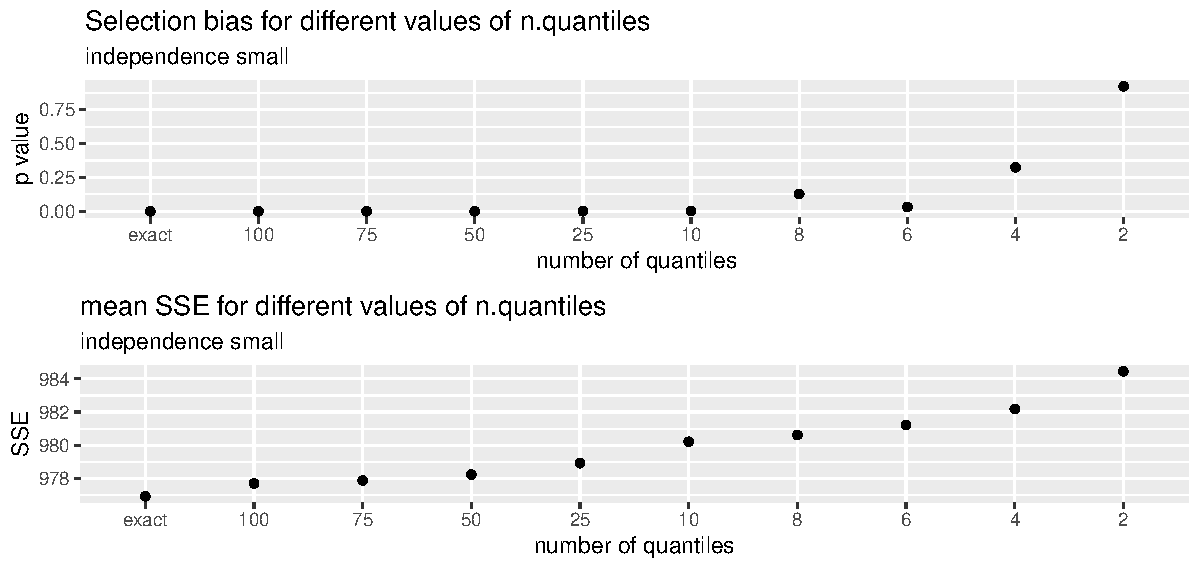
\includegraphics[width=10cm]{Figures/simulations/batchtools/selection_bias_slim/independence_small.pdf}
\end{figure}
\end{frame}

\begin{frame}{Influence of n.quantiles in SLIM on selection bias and performance}
$X_1$ and $X_2 \sim U(0,1)$; $X_3$ binary\\
$Y = X_1 + X_2 + X_3 + 0.01X_1X_2 + \epsilon$

\begin{table}

\caption{frequency of selecting covariate Xi as splitting variable}
\centering
\begin{tabular}[t]{l|r|r|r|r|r|r|r|r|r|r}
\hline
  & exact & 100 & 75 & 50 & 25 & 10 & 8 & 6 & 4 & 2\\
\hline
x1 & 502 & 487 & 504 & 510 & 494 & 502 & 505 & 480 & 502 & 483\\
\hline
x2 & 497 & 511 & 494 & 488 & 504 & 495 & 491 & 512 & 485 & 433\\
\hline
x3 & 1 & 2 & 2 & 2 & 2 & 3 & 4 & 8 & 13 & 84\\
\hline
\end{tabular}
\end{table}

$\Rightarrow$ When n.quantiles is very small, the binary variable without actual interaction effect is more often mistakenly chosen as splitting variable

\end{frame}

\begin{frame}{Influence of n.quantiles in SLIM on selection bias and performance}
$X_1$ and $X_2 \sim U(0,1)$; $X_3$ categorical with 5 classes\\
$Y = X_1 + X_2 + X_3 + 0.01X_1X_2 + \epsilon$

\begin{table}

\caption{frequency of selecting covariate Xi as splitting variable}
\centering
\begin{tabular}[t]{l|r|r|r|r|r|r|r|r|r|r}
\hline
  & exact & 100 & 75 & 50 & 25 & 10 & 8 & 6 & 4 & 2\\
\hline
x1 & 507 & 507 & 510 & 509 & 518 & 492 & 490 & 489 & 466 & 442\\
\hline
x2 & 493 & 493 & 490 & 491 & 481 & 504 & 507 & 504 & 521 & 440\\
\hline
x3 & 0 & 0 & 0 & 0 & 1 & 4 & 3 & 7 & 13 & 118\\
\hline
\end{tabular}
\end{table}
\end{frame}




\begin{frame}{Next Steps}
\begin{enumerate}
    \item Writing of the first three chapters (Introduction, Related Work, Methodology)
    \item Implementation of Guide bootstrap correction bias 
    \item Finishing simulations regarding selection bias (possibly write down results)
    \item Definition of a stability measure and implementation of its calculation
    \item Definition of scenarios for the comparison of performance, stability and interpretability
\end{enumerate}
    
\end{frame}
    


\begin{frame}{Bibliography}
    \bibliography{bibliography}
    \bibliographystyle{dcu}

\end{frame}
\end{document}




